\documentclass[11pt, a4paper]{report}

\usepackage[T1]{fontenc} 								
\usepackage[norsk]{babel}								
\usepackage[utf8]{inputenc}						
\usepackage{graphicx}       						
\usepackage{amsmath,amssymb}
\usepackage{grffile}
\usepackage{listings}
\usepackage{caption}
\usepackage[export]{adjustbox}
\usepackage{titling}
\setcounter{secnumdepth}{0}

\lstset{extendedchars=true, basicstyle=\footnotesize, numbers=left, numberstyle=\tiny, frame=shadowbox, tabsize=2, language=C, showstringspaces=false, breaklines=true,
  literate=
  {á}{{\'a}}1 {é}{{\'e}}1 {í}{{\'i}}1 {ó}{{\'o}}1 {ú}{{\'u}}1
  {Á}{{\'A}}1 {É}{{\'E}}1 {Í}{{\'I}}1 {Ó}{{\'O}}1 {Ú}{{\'U}}1
  {à}{{\`a}}1 {è}{{\`e}}1 {ì}{{\`i}}1 {ò}{{\`o}}1 {ù}{{\`u}}1
  {À}{{\`A}}1 {È}{{\'E}}1 {Ì}{{\`I}}1 {Ò}{{\`O}}1 {Ù}{{\`U}}1
  {ä}{{\"a}}1 {ë}{{\"e}}1 {ï}{{\"i}}1 {ö}{{\"o}}1 {ü}{{\"u}}1
  {Ä}{{\"A}}1 {Ë}{{\"E}}1 {Ï}{{\"I}}1 {Ö}{{\"O}}1 {Ü}{{\"U}}1
  {â}{{\^a}}1 {ê}{{\^e}}1 {î}{{\^i}}1 {ô}{{\^o}}1 {û}{{\^u}}1
  {Â}{{\^A}}1 {Ê}{{\^E}}1 {Î}{{\^I}}1 {Ô}{{\^O}}1 {Û}{{\^U}}1
  {ã}{{\~a}}1 {Ã}{{\~A}}1 {õ}{{\~o}}1 {Õ}{{\~O}}1
  {œ}{{\oe}}1 {Œ}{{\OE}}1 {æ}{{\ae}}1 {Æ}{{\AE}}1 {ß}{{\ss}}1
  {ç}{{\c c}}1 {Ç}{{\c C}}1 {ø}{{\o}}1 {å}{{\r a}}1 {Å}{{\r A}}1
  {€}{{\EUR}}1 {£}{{\pounds}}1}

\setlength{\textheight}{240mm} 
\setlength{\textwidth}{180mm}  
\topmargin -5mm 
\oddsidemargin -5mm
\captionsetup[figure]{singlelinecheck=off, justification = raggedleft} 
\pretitle{%
  \begin{center}
  \LARGE
  
\includegraphics[width=6cm,height=6cm]{uitlogo.png}\\[\bigskipamount]
}
\posttitle{\end{center}}

\begin{document}

\title{Hastighet til modellbil ned skråplan}
\author{Fredrik Sandhei \thanks{UiT - AUT-1001, obligatorisk innlevering 1}}
\date{\today}
\maketitle
\newpage
\tableofcontents
\newpage

\section{Introduksjon}
Denne rapporten er en besvarelse på den første obligatoriske innleveringen i faget AUT-1001, i samsvar med å lære seg å bruke 8-bits mikrokontrolleren ATmega16 med STK-500-brettet for ISP (In-System Programming). Oppgaven skulle løses med å lage et C-program i IDE Atmel Studio, som fant hastigheten til en modellbil ned et skråplan. 

\section{Hensikt}
Hensikten med denne oppgaven var å undersøke gyldigheten til den såkalte 'tidsløse formelen' $ 2as = v^{2} - v_{0}^{2} $ med hjelp av sensorer for å måle tiden, og dermed hastigheten til modellbilen og sjekke den opp mot teorien.

\section{Teori}
Fra fysikken har man ved hjelp av tiden $t$ og akselerasjonen $a$ muligheten til å finne et uttrykk for hastigheten $v$ til et objekt som beveger seg. Ved hjelp av integrasjon av (\ref{hastighet}) får en uttrykt strekning avlagt $x$ ved tiden $t$.

\begin{equation} \label{hastighet}
v = v_{0} + at
\end{equation}
\begin{equation} \label{strekning}
x = x_{0} + v_{0}t + \frac{1}{2}at^{2}
\end{equation}
Substituerer man t fra (\ref{hastighet}) og setter den inn i (\ref{strekning})får man hastigheten uttrykt uavhengig av tid.

\begin{equation}
2as = v^{2}-v_{0}^{2} \implies v^{2} = 2as-v_{0}^{2}
\end{equation}
\newline

I dette tilfellet skulle bilen rulle ned et skråplan med en fritt bestemt helning $\alpha$. Akselerasjonen til bilen blir bestemt ut i fra tyngdeakselerasjonen samt vinkelen mellom relativ bevegelsesretning og horisontal akse, og er dermed gitt ved $a = gsin \alpha$. Fra uttrykket og figuren under er det klart at ved høyere vinkel ($0^\circ \leq\alpha\leq 90^\circ$) får en høyere akselerasjon og dermed høyere hastighet.\newline

For å kunne måle hastigheten kan en ved hjelp av eksterne interrupts koblet til tre IR-sensorer og timer/counter finne tiden det tar for at modellbilen bryter to IR-lyssensorer.
Hensikten med å bruke interrupts er at de stopper opp programmet som mikrokontrolleren kjører og gjennomfører en Interrupt Service Protocol (ISP) dersom det er en bestemt tilstandsendring som oppstår.\newline For denne problemstillinga ble det brukt en 16-bits timer, timer1, som kan telle, tilbakestilles og stoppes, men brukes også i sammenheng med ICP - Input Capture Pin - for å måle tiden mellom to like logiske nivåendringer. 
Sensor $S_{1}$ er koblet til pd2 på mikrokontrolleren, som har INT0(External Interrupt 0) som spesialfunksjon. Når pin 2 på port D blir satt høy, blir en ISP for INT0 gjennomført. Da blir det registrert at et objekt (slik som denne modellbilen) kommer ned skråplanet. Når ICP på pin 6 på port D, som er koblet til sensorene $S_{2}$ og $S_{3}$, går høy, blir timeren tilbakestilt, i tillegg til eventuelle overflows fra TIMER1-interrupten (antall ganger klokken har passert maksverdi - 65535). Tida det går fra timeren er tilbakestilt og en ending edge blir registrert i Input Capture - registeret, blir da tida det tok å passere $S_{2}$ og $S_{3}$. Avstanden mellom $S_{2}$ og $S_{3}$ er på 10cm.\newline Da 16-bits timeren går på samme klokkefrekvens som mikrokontrollerens prosessor ($F_{CPU} = 3686400 Hz$), er det praktisk å senke hastigheten til timer-klokka. Dette oppnås ved prescalers, der klokkehastigheten kan enten reduseres med en 1,8,64,256,1024-divider. I denne løsningen ble en 8-divider brukt som prescaler.

\begin{figure}
  \centering
  \captionbox
  {Det hjemmelagde skråplanet av foreleseren, med $S_{2}$ og $S_{3}$ fremst, og $S_{1}$ bakerst.}
  {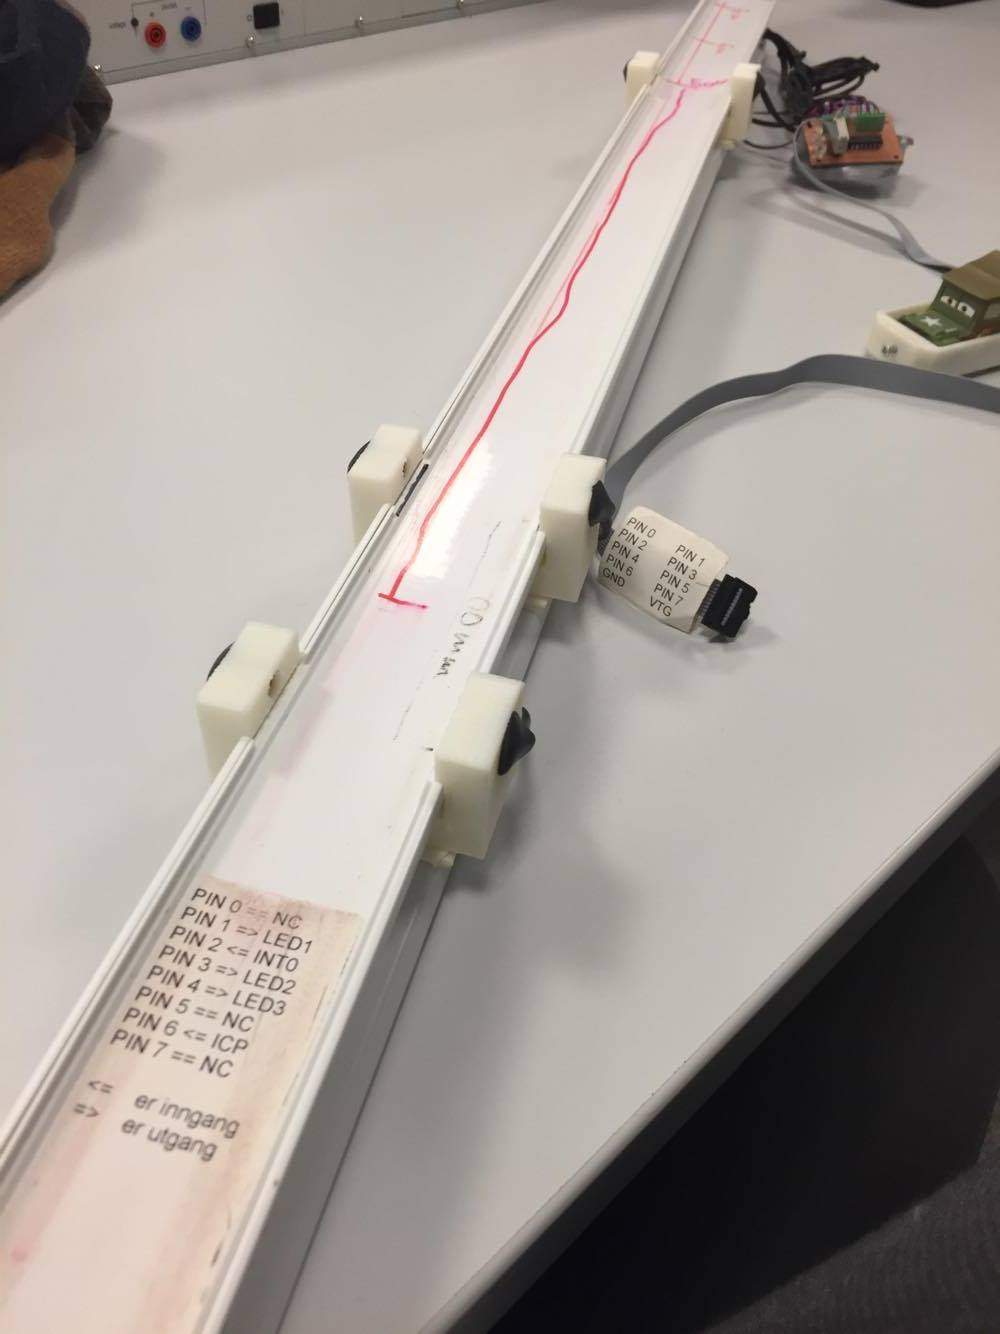
\includegraphics[width=0.4\textwidth, right]{field.jpg}}
\end{figure}

\section{Løsning}
\subsection{Tilstandsmaskin}
Ved hjelp av den eksterne interrupten INT0 kan man lage en tilstandsmaskin (Finite-State Machine, eller FSM), der mikrokontrolleren gjennomfører ulike operasjoner for TIMER1-ICP-interruptene basert på tilstanden den er i. Tilstanden endres ved hjelp av de ulike sensorene. På denne måten vil ikke en ny tid bli målt før bilen passerer $S_{1}$ på nytt. Dessuten blir det også lettere å skrive koden, da man må bare lete etter hvilken tilstand mikrokontrolleren er i ved gitt tidspunkt. 

\subsection{Implementering av tilstandsmaskinen}
Utgangspunktet for tilstandsmaskinen er følgende: Registrer at bilen er i bevegelse og tilbakestill registrert hastighet. Start TIMER1 og telle fram til $S_{2}$. Ved $S_{2}$, nullstill overflow-telleren $ov\_counter$ og timer1 $TCNTR1$, men fortsette å telle, og endre tilstandsvariabelen($running = 2;$). I denne tilstanden vil mikrokontrolleren vente til en ending edge oppstår, og legger til antall klokketikker fra overflowene dersom det var noen. Ettersom $clocks$ - variabelen finner antall klokketikker siden den siste ending edge, dvs siste gang ICP ble høy, blir tiden det tok fra $S_{2}$ og $S_{3}$ å dividere $clocks$ på timer1-frekvensen. Hastigheten blir da beregnet med $v = s/t$, der $ s = distance = 100mm$.\newline

Resultanthastigheten skrives så ut på en syvsegmentsskjerm gjennom unsigned-char-funksjonen \newline $displaySpeed()$, med hastigheten som argument. Da output på skjermen var regulert ved å sette relaterte bits til de ulike ledlysene høy, blir det komplisert å innblande floats/desimaltall. Dessuten blir det mer minne å bruke, da denne datatypen bruker 64 bits, i motsetning til int på 16 bits. Derfor ble hastigheten økt med graden 10. Det første sifferet blir da hastighet heltallsdividert på 10, og det siste sifferet hastighet modulo 10. For å skille det første og siste sifferet fra hverandre, blir det første sifferet OR-ed med 1, da det 0. bit er reservert til desimalet. 


\begin{figure}[htbp]
	\begin{center}
		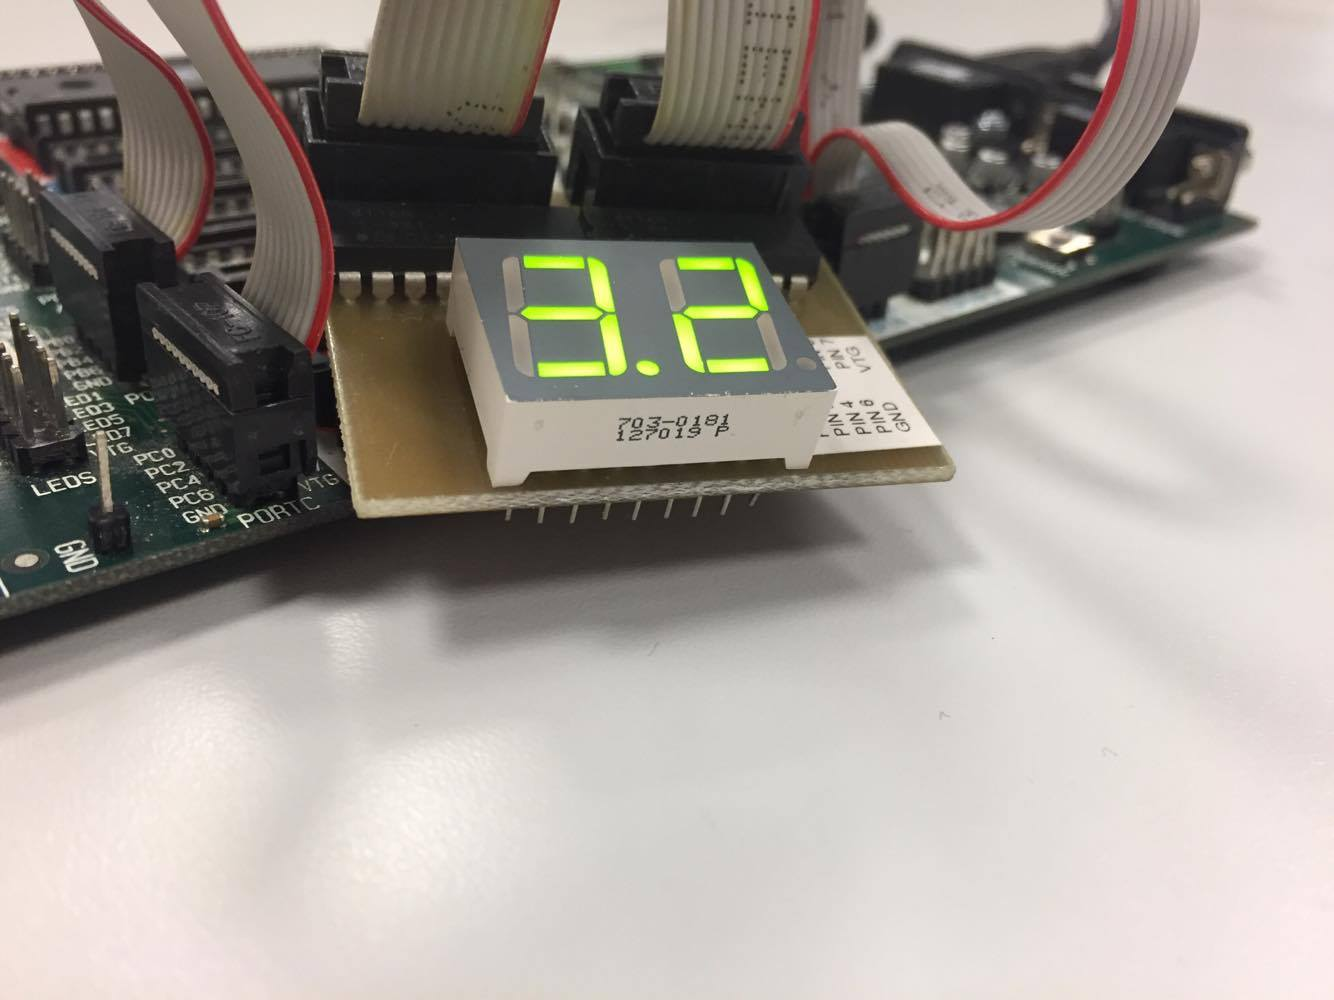
\includegraphics[width=0.4\textwidth, right]{display.jpg}
		\caption{Syvsegmentsskjermen brukt.}
	\end{center}
\end{figure}

\section{Testing}
I denne seksjonen vises testresultatene med ulik $\alpha$ satt opp mot den teoretiske (gjennom (\ref{hastighet})) og den praktiske. Da vinkelen ikke blir nøyaktig ønsket, blir det en liten feilkilde, da for eksempel $\pm$ 5 graders forskjell gir en forskjell på $\pm$ 0.3 m/s. For målingene ble det prøvd tre ganger for hver $\alpha$, og deretter gjennomsnittet av disse blir vist. Den totale strekningen for bilen hver runde var $550mm$.

\begin{table}[h]
\caption{Teoretisk hastighet mot praktisk hastighet med ulike $\alpha$ og $F_{CPU_{8}}$}
\begin{center}
\begin{tabular}{ccccc}
\hline
Vinkel ($\alpha$)  & Teoretisk ($ v =\sqrt{2as}$) &  Praktisk\\
\hline

$\alpha = 30^{\circ}\rm$ & $2.3 m/s\rm$ & ($2.0 \pm 0.3) m/s \rm$\\

$\alpha = 40^{\circ}\rm$ & $2.6 m/s\rm $& ($2.3 \pm 0.3) m/s \rm $ \\

$\alpha = 60^{\circ}\rm$ & $3.0 m/s\rm $& ($2.7\pm 0.3) m/s \rm $ \\

\hline

\end{tabular}
\end{center}
\end{table}




\section{Resultater}

Fra testene virker det som om at hastigheten som måles har et avvik på ca $0.3 m/s$ under den hastigheten som 'forventes' fra teorien. Til tross for avviket, ble resultatet omtrent som forventet: Jo høyere $\alpha$, desto høyere hastighet oppnår man. Det virket også om hastigheten målt ble stadig mer nøyaktig da $\alpha$ ble tilstrekkelig stor. Antageligvis har dette noe sammenheng med friksjonskrafta som bilen opplever fra underlaget, som tilsynelatende påvirket resultatet betydelig.
 
\section{Diskusjon}

Den 'tidsløse' hastighetformelen $v = \sqrt{2as}$, hvor $a = g\cdot sin\alpha$, ikke tar hensyn til ytre påvirkninger, slik som luftmotstand (forsåvidt neglisjerbar) og friksjon mellom legemet og underlaget. Dermed ble den målte hastigheten noe mindre enn fra formelen. Den vinkelen som ble satt har også sine feilmarginer, da den kan veksle litt mellom høyere og lavere verdier. Det viser seg gjennom litt regning at en $\pm 5^{\circ}$ forskjell fra ønsket vinkel, ville hastigheten endres med $\pm$ 0.3 m/s, dersom vinklene var tilstrekkelig små ($0^\circ \leq\alpha\leq 60^\circ$). En annen faktor er strekninga bilen tilbakela. Antageligvis er denne forskjellen for hver runde neglisjerbar.
\newline
Dersom man kunne velge et annet underlag, for eksempel en luftputebane, kunne friksjonen neglisjeres og da vil den målte hastigheten bli tilnærmet lik den teoretiske. Videre ville jeg ha endret programmet til å få TIMER1 - klokken stoppet frem til ICP blir høy, for å ikke kaste bort minne på tid som ikke deltar i målingen. Noe annet kan være å få satt en avstandssensor på banen for å kunne forsikre at man testet med lik strekning for hver runde. 
\newline

En nevneverdig sak, men en liten avsporing, er beregning av selve hastigheta (se vedlegget). Hastigheta ble multiplisert med 10 for å ikke rote med floats, men eksakt ''hvor'' en skulle multiplisere med 10 var ikke ''bare, bare'': Dersom man lot hastigheten være på formen
\begin{lstlisting}
	speed = ((unsigned long)distance/finish_time)*10;
\end{lstlisting}
i stedet for
\begin{lstlisting}
	speed = (unsigned long)(distance*10/finish_time);
\end{lstlisting}
ville ikke hastigheten bli riktig vist ut på skjermen. Grunnen til dette ligger i C-operatoren $/$, som er heltallsdivisor. Det vil si at den runder opp til det nærmeste minste hele tallet. Da vil den første $speed$ - eksempelet vise bare $0$ som desimaltall, mens den andre vil vise mer eller mindre korrekt hastighet. 


\section{Konklusjon}
Koden implementert for dette problemet var basert på en tilstandsmaskin, slik at man lettere observere eventuelle feilkilder ved feilkilder. Tilstandsmaskinen funket godt til denne problemstillingen. Hastighetene hadde noe avvik fra den tidløse hastighetsformelen, men faktorer som unøyaktige vinkler, friksjonskrefter og luftmotstand påvirker resultatet. Likevel kan man være fornøyde med utfallet. 

\newpage
\section{Vedlegg}

\lstinputlisting{main.c}
\end{document}

